%%%%%%%%%%%%%%%%%%%%%%%%%%%%%%%%%%%%%%%%%
% Masters/Doctoral Thesis 
% LaTeX Template
% Version 1.41 (9/9/13)
%
% This template has been downloaded from:
% http://www.latextemplates.com
%
% Original authors:
% Steven Gunn 
% http://users.ecs.soton.ac.uk/srg/softwaretools/document/templates/
% and
% Sunil Patel
% http://www.sunilpatel.co.uk/thesis-template/
%
% License:
% CC BY-NC-SA 3.0 (http://creativecommons.org/licenses/by-nc-sa/3.0/)
%
% Note:
% Make sure to edit document variables in the Thesis.cls file
%
%%%%%%%%%%%%%%%%%%%%%%%%%%%%%%%%%%%%%%%%%

%----------------------------------------------------------------------------------------
%	PACKAGES AND OTHER DOCUMENT CONFIGURATIONS
%----------------------------------------------------------------------------------------

\documentclass[11pt, a4paper, oneside]{Thesis} % Paper size, default font size and one-sided paper

\graphicspath{{Pictures/}} % Specifies the directory where pictures are stored

\usepackage{verbatim}
\usepackage[square, numbers, comma, sort&compress]{natbib} % Use the natbib reference package - read up on this to edit the reference style; if you want text (e.g. Smith et al., 2012) for the in-text references (instead of numbers), remove 'numbers' 
\usepackage{algorithm}
\usepackage{algorithmic}
\hypersetup{urlcolor=blue, colorlinks=true} % Colors hyperlinks in blue - change to black if annoying
\title{\ttitle} % Defines the thesis title - don't touch this

\begin{document}

\frontmatter % Use roman page numbering style (i, ii, iii, iv...) for the pre-content pages

\setstretch{1.3} % Line spacing of 1.3

% Define the page headers using the FancyHdr package and set up for one-sided printing
\fancyhead{} % Clears all page headers and footers
\rhead{\thepage} % Sets the right side header to show the page number
\lhead{} % Clears the left side page header

\pagestyle{fancy} % Finally, use the "fancy" page style to implement the FancyHdr headers

\newcommand{\HRule}{\rule{\linewidth}{0.5mm}} % New command to make the lines in the title page

% PDF meta-data
\hypersetup{pdftitle={\ttitle}}
\hypersetup{pdfsubject=\subjectname}
\hypersetup{pdfauthor=\authornames}
\hypersetup{pdfkeywords=\keywordnames}

%----------------------------------------------------------------------------------------
%	TITLE PAGE
%----------------------------------------------------------------------------------------

\begin{titlepage}
\begin{center}

\textsc{\LARGE Imperial College of London}\\[1.5cm] % University name
\textsc{\Large Research Project Report}\\[0.5cm] % Thesis type

\HRule \\[0.4cm] % Horizontal line
{\huge \bfseries Learning Music Representation using Recurrent Neural Networks}\\[0.4cm] % Thesis title
\HRule \\[1.5cm] % Horizontal line
 
\begin{minipage}{0.4\textwidth}
\begin{flushleft} \large
\emph{Author:}\\
Clement Jambou% Author name - remove the \href bracket to remove the link
\end{flushleft}
\end{minipage}
\begin{minipage}{0.4\textwidth}
\begin{flushright} \large
\emph{Supervisor:} \\
\supname % Supervisor name - remove the \href bracket to remove the link  
\end{flushright}
\end{minipage}\\[3cm]
 
%\large \textit{A thesis submitted in fulfilment of the requirements\\ for the degree of \degreename}\\[0.3cm] % University requirement text
%\textit{in the}\\[0.4cm]
%\groupname\\\deptname\\[2cm] % Research group name and department name
 


\includegraphics[scale=0.4]{Figures/Logo} % University/department logo - uncomment to place it


{\large \today}\\[4cm] % Date 
\vfill
\end{center}

\end{titlepage}
\clearpage
%----------------------------------------------------------------------------------------
%	DECLARATION PAGE
%	Your institution may give you a different text to place here
%----------------------------------------------------------------------------------------
\begin{comment}
\Declaration{

\addtocontents{toc}{\vspace{1em}} % Add a gap in the Contents, for aesthetics

I, \authornames, declare that this thesis titled, '\ttitle' and the work presented in it are my own. I confirm that:

\begin{itemize} 
\item[\tiny{$\blacksquare$}] This work was done wholly or mainly while in candidature for a research degree at this University.
\item[\tiny{$\blacksquare$}] Where any part of this thesis has previously been submitted for a degree or any other qualification at this University or any other institution, this has been clearly stated.
\item[\tiny{$\blacksquare$}] Where I have consulted the published work of others, this is always clearly attributed.
\item[\tiny{$\blacksquare$}] Where I have quoted from the work of others, the source is always given. With the exception of such quotations, this thesis is entirely my own work.
\item[\tiny{$\blacksquare$}] I have acknowledged all main sources of help.
\item[\tiny{$\blacksquare$}] Where the thesis is based on work done by myself jointly with others, I have made clear exactly what was done by others and what I have contributed myself.\\
\end{itemize}
 
Signed:\\
\rule[1em]{25em}{0.5pt} % This prints a line for the signature
 
Date:\\
\rule[1em]{25em}{0.5pt} % This prints a line to write the date
}

\clearpage % Start a new page
\end{comment}
\clearpage % Start a new page

%----------------------------------------------------------------------------------------
%	ABSTRACT PAGE
%----------------------------------------------------------------------------------------

\addtotoc{Abstract} % Add the "Abstract" page entry to the Contents

\abstract{\addtocontents{toc}{\vspace{1em}} % Add a gap in the Contents, for aesthetics

    It is a widely known assumption that creativity to produce art and algorithmic are incompatible. In many science fiction movies one of the major differences between an AI and humans is its capacity for creativity. In this project, we focus on the problem of training artificial recurrent neural networks. Recurrent Neural Networks are a powerful model to learn complex sequence, like (classical) music. We describe music scores as a sequence of notes, that take values in a finite set and with a discrete representation of time. A music melody contains many rules that depends for instance of its composer among other things. This set of rules, or patterns can have different time scales. For example, it is often the case in classical music that a phrase ( a subsequence of the score ) will end with an harmonic cadence, constraining its last two notes. Another example is the fact that a specific theme can be heard in the begining and in the end of a piece. Because of this large set of rules it is hard for most humans to compose music, though their "musical ear" are trained in an unsupervised way to hear what seems "natural" or "unnatural". In many ways this set of rules can be compared to the syntax of a natural language. This complexity within the musical patterns makes it a good natural problem that can be used as a benchmark for training Recurrent Neural Networks.   

    In this project, the goal is to propose improvements on the training of a Recurrent Neural Network to achieve a good performance on different benchmarks. A databse of MIDI files is one of these benchmarks, where we can quantify the score of the network as well as hear its production and evaluate its achievements qualitatively. To do so we use a set of music scores (through MIDI files) to learn an abstract version of these rules and use the generative properties of the network to produce music. By predicting the value of the next note in a sequence, it is possible to evaluate how the network performs in understanding a set of music scores, and focus on minimizing this undersanding on a test set. 

}

\clearpage % Start a new page

%----------------------------------------------------------------------------------------
%	ACKNOWLEDGEMENTS
%----------------------------------------------------------------------------------------

\setstretch{1.5} % Reset the line-spacing to 1.3 for body text (if it has changed)

%\acknowledgements{\addtocontents{toc}{\vspace{1em}} % Add a gap in the Contents, for aesthetics

%Professor Emmanuel Rachelson, Department of Mathematics, Computing and Automation, Supaero Graduate Program ISAE, Toulouse

%The acknowledgements and the people to thank go here, don't forget to include your project advisor\ldots
%}
\clearpage % Start a new page

%----------------------------------------------------------------------------------------
%	LIST OF CONTENTS/FIGURES/TABLES PAGES
%----------------------------------------------------------------------------------------

\pagestyle{fancy} % The page style headers have been "empty" all this time, now use the "fancy" headers as defined before to bring them back

\lhead{\emph{Contents}} % Set the left side page header to "Contents"
\tableofcontents % Write out the Table of Contents

\lhead{\emph{List of Figures}} % Set the left side page header to "List of Figures"
\listoffigures % Write out the List of Figures

%\lhead{\emph{List of Tables}} % Set the left side page header to "List of Tables"
%\listoftables % Write out the List of Tables

%----------------------------------------------------------------------------------------
%	ABBREVIATIONS
%----------------------------------------------------------------------------------------
\begin{comment}
\clearpage % Start a new page

\setstretch{1.5} % Set the line spacing to 1.5, this makes the following tables easier to read

\lhead{\emph{Abbreviations}} % Set the left side page header to "Abbreviations"
\listofsymbols{ll} % Include a list of Abbreviations (a table of two columns)
{
\textbf{LAH} & \textbf{L}ist \textbf{A}bbreviations \textbf{H}ere \\
%\textbf{Acronym} & \textbf{W}hat (it) \textbf{S}tands \textbf{F}or \\
}

%----------------------------------------------------------------------------------------
%	PHYSICAL CONSTANTS/OTHER DEFINITIONS
%----------------------------------------------------------------------------------------

\clearpage % Start a new page

\lhead{\emph{Physical Constants}} % Set the left side page header to "Physical Constants"

\listofconstants{lrcl} % Include a list of Physical Constants (a four column table)
{
Speed of Light & $c$ & $=$ & $2.997\ 924\ 58\times10^{8}\ \mbox{ms}^{-\mbox{s}}$ (exact)\\
% Constant Name & Symbol & = & Constant Value (with units) \\
}

%----------------------------------------------------------------------------------------
%	SYMBOLS
%----------------------------------------------------------------------------------------

\clearpage % Start a new page

\lhead{\emph{Symbols}} % Set the left side page header to "Symbols"

\listofnomenclature{lll} % Include a list of Symbols (a three column table)
{
$a$ & distance & m \\
$P$ & power & W (Js$^{-1}$) \\
% Symbol & Name & Unit \\

& & \\ % Gap to separate the Roman symbols from the Greek

$\omega$ & angular frequency & rads$^{-1}$ \\
% Symbol & Name & Unit \\
}

%----------------------------------------------------------------------------------------
%	DEDICATION
%----------------------------------------------------------------------------------------

\setstretch{1.3} % Return the line spacing back to 1.3

\pagestyle{empty} % Page style needs to be empty for this page

\dedicatory{For/Dedicated to/To my\ldots} % Dedication text

\addtocontents{toc}{\vspace{2em}} % Add a gap in the Contents, for aesthetics

\end{comment}
%----------------------------------------------------------------------------------------
%	THESIS CONTENT - CHAPTERS
%----------------------------------------------------------------------------------------

\mainmatter % Begin numeric (1,2,3...) page numbering

\pagestyle{fancy} % Return the page headers back to the "fancy" style

% Include the chapters of the thesis as separate files from the Chapters folder
% Uncomment the lines as you write the chapters

% Chapter Template

\chapter{Introduction} % Main chapter title

\label{Chapter 1} % Change X to a consecutive number; for referencing this chapter elsewhere, use \ref{ChapterX}

\lhead{Chapter 1. \emph{Related Work}} % Change X to a consecutive number; this is for the header on each page - perhaps a shortened title

%----------------------------------------------------------------------------------------
%	SECTION 1
%----------------------------------------------------------------------------------------

%\section{State of the Art}

\section{Motivation}
\section{Aims}
\section{Contributions}


% Chapter Template

\chapter{Related Work} % Main chapter title

\label{Chapter 1} % Change X to a consecutive number; for referencing this chapter elsewhere, use \ref{ChapterX}

\lhead{Chapter 1. \emph{Related Work}} % Change X to a consecutive number; this is for the header on each page - perhaps a shortened title

%----------------------------------------------------------------------------------------
%	SECTION 1
%----------------------------------------------------------------------------------------

%\section{State of the Art}

\section{Overview}

Over the last two decades, the focus of the Machine Learning community on deep learning, (ie the study of Deep Neural Networks) has grown considerably. Because of the hardware improvements as well as several improvement of the optimization techniques, Neural Networks outperforms other Machine Learning techniques in many domains and applications where they have won several competitions. Escpecially when it concerns problems with large set of input features or complex sequential relations (for instance in Computer Vision, or voice recognition). It is therefore natural to use the approach of training a Recurrent Neural Network to learn the music representation as this approach has been sucessful in solving similar problems. In the following, we will detail some of the achievements and techniques used with Neural Networks to motivate and justify this choice. The recent survey paper of Schmidhuber et al. \cite{schmidhuber2014deep} and Bengio et al.\cite{bengio2013advances} was very useful in the orientation of the relevant related work. 

\newpage
\section{Recurrent Neural Network}

Artificial Neural Networks (ANNs) were introduced in the 1940s (e.g., McCulloch and Pitts, 1943) in an attempt to model the functionning of the brain, even if the first models are inspired of linear regression introduced by mathematicians like Gauss and Legendre in the 19th centery. An artificial neural network contains a graph, where the nodes are representing neurons. A neuron can be an input neuron, directly connected to an input from a sensor or a dataset, a hidden neuron with different inputs from other neurons or an output neuron, also with different inputs from neurons, but from which it is possible to read a value. Different models have been built to model the interaction between neurons. These models can be inspired directly from biology (for instance in the hodgkin-huxley model \cite{lytton2002hodgkin}). For the specific use of Machine Learning problems however, the model of the neurons is simplified to be able to use large networks of neurons and the backpropagation algorithm. The classical form of the neuron is as follow : 
$$ out = a (W * X + b)$$ where, $W$ it the weight matrix and $b$ a bias vector. $a$ is called the activation function and can be used to introduce non-linearity in the model.
Classical activation functions have sigmoid shape like hyperbolic tangent or the logistic function ($ \frac 1 {1 + \exp x}$).
Lately however the use of rectified linear unit (ReLU): $$a(x) = max(x, 0)$$ have shown significant improvement for some applications (mainly for calculation speed reasons \cite{dahl2013improving})  
It is possible to use this equation to update a set of neurons directly and simplify the notation using matrix notations. 

The model of the Feedforward Neural Networks (FNN), with no recurrent connection (ie no loops) can be described as follow:

$$
\begin{array}{rcr} 
    h_0 & = & x \\h_i & = & a ( W_{i} * h_{i-1}) \\ \hat{y} & = & h_n
\end{array}
$$

where the set of neurons is organised in layer ($n$ is the number of layers and $h_i$ is the output of the $i_{th}$ layer ). The shapes of the weight matrix $W_i$ describe the topology of the graph of neurons, ie the architecture of neural network. FNNs are an improvement of the logistic regression model (a network with 1 layer). It is possible to learn the weights matrices and biases using gradient descent. The success of the FNN model comes from the backpropagation algorithm, witch enables to compute the gradient of the error of the model  $error = D(y, \hat{y})$ where D is a distance function between the prediction of the network and the real value to be predicted. The gradient is computed over the set of parameters (ie the weights and biases) efficiently using the function composition gradient (backward propagation of the error).

A Recurrent Neural Network (RNN) is a more general type of network where loops in the connection are allowed. Because of the loops, it is not possible to use the backpropagation algorithm in the same way as for Feedforward Neural Networks. For the same reason it is convenient to introduce a time dependency in RNNs (some neurons may have states that don't converge). The equation describing a Recurrent Neural Network can be written as follow : 


Given a sequence of inputs: $x_1, x_2, ... x_t$ and the hidden states $h_1, h_2, ..., h_t$.
$$
\begin{array}{rcr} 
    h_0 & = & a(W_{hx}  * x_0 + b_{init} + b_h)  \\ 
    h_i & = & a(W_{hx}  * x_i + W _{hh} * h_{i-1} + b_h)  \\ 
    \hat{y}_i & = & a'(W_{yh} + b_y)

\end{array}
$$

\begin{figure}[htbp]
    \centering
    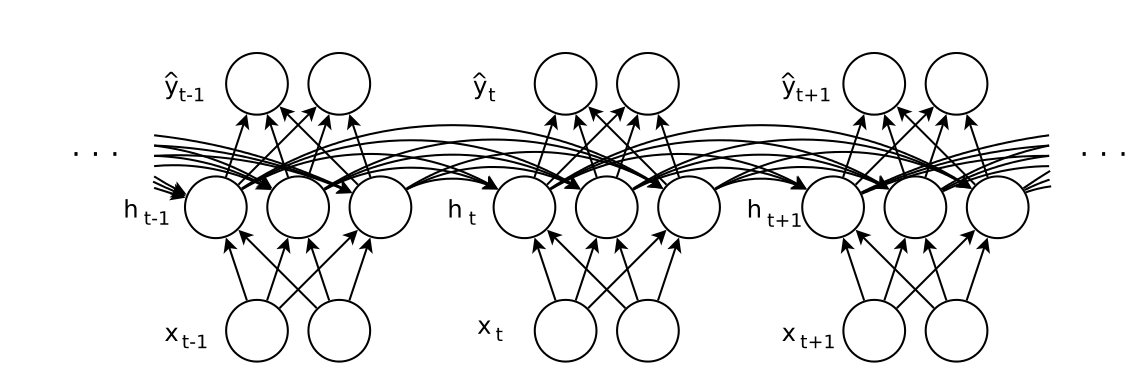
\includegraphics[scale=0.3]{Figures/RNN.png}
    \rule{35em}{0.5pt}
    \caption[Recurrent Neural Network]{Recurrent Neural Network}
    \label{fig:rnn}
\end{figure}




We generate a set of predictions ($\hat{y}_1, \hat{y}_2, ... \hat{y}_t$) from the network. The architecture is described with the shapes of the weight matrix $W_{hx}$ (input to hidden), $W_{hh}$ (hidden to hidden) and $W_{yh}$ (hidden to output). The parameters of the network are the weights and the biases ($b_h$, $b_{init}$, $b_y$).
We can consider this network as a special kind of very deep Feed Forward Network, where each time step has its own layer and with constraints on the weights. With this analogy it is possible to build a version of the backpropagation algorithm for Recurrent Neural Networks called Backpropagation trough time \cite{werbos1990backpropagation}.


\section{Hessian Free Optimization}

Efficiently training a Neural Network remains an area of focus of the Machine Learning community. In the 1990s, this problem seemed impossible to solve for real applications and many machine learning researcher prefered other methods. In the last decade, the progress of computation power, as well as implementation of fast matrix calculation on Graphics Processing Units (GPU) made it possible for neural network to be trained $10^6$ time faster. But the progress of computation is not the only reason for the sucess of Neural Networks today. Many improvements in the model, such as Hinton et al. dropouts \cite{dahl2013improving}, implementation of convolutional neural network on GPU \cite{krizhevsky2012imagenet} or the introduction of Long Short Term Memory Recurrent Neural Networks (LSTM, hochreiter et al. \cite{hochreiter1997long}) and on the optimization method where introduced. One of the major issue with standard stochastic gradient descent when applied to deep Neural Networks, and therefore to Recurrent Neural Networks is the called exploding vanishing gradient. When evaluating the gradient of the error of the network on the weight, because of the derivative of the composition of 2 functions, products of weights appear in the calculations of the gradient. When the network is deep, is can be shown that this product of weights grows exponentially \cite{pascanu2012difficulty}. The difference between the gradient on different direction in the parameters space makes it harder for the gradient descent to converge. To undestand this phenomena, we can consider the gradient descent applied to a problem where the equipotential are flat ellipses. The direction given by the gradient will be toward the largest axis of the elipse, and it will take many steps to converge toward the center of the elipse. In the opposite if the equipotential is a circle, then the direction given by the gradient is the best. 


\begin{figure}[htbp]
    \centering
    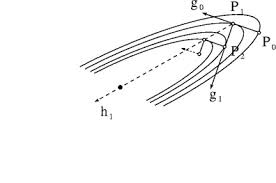
\includegraphics[scale=0.7]{Figures/gradient_ellipse.jpg}
    \rule{35em}{0.5pt}
    \caption[Difficulty of gradient descent]{Difficulty of gradient descent}
    \label{fig:gradient_elipse}
\end{figure}

In order for the gradient direction to be less dependant to linear transformation of the parameter space, we need to look at higher order of derivatives. Applying newton's method to $\phi(X)$ is the same as applying it to $\phi(A*X)$ for $A$ invertible. However, newton's method requires to inverse the curvature matrix, which is not computationally feseable, event for medium size networks. Several techniques used in optimization perform lower rank approximation (L-BFGS) of the curvature matrix in order to solve this issue. However, these approximations are not satisfactory for deep neural networks, because the approximation will be to influenced by the exploding and vanishing gradient. In 2010, Martens et al. proposed several modification to the Hessian Free Optimization techniques in order to apply them to Deep Neural Networks \cite{martens2010deep} and to Recurent Neural Networks \cite{martens2011learning}. 

The Hessian Free Optimization method, like the gradient descent is an iterative process. It takes into account the curvature (ie the second order derivative) of the fitness function, but does not require the inversion of the matrix nor any approximation of the curvature. At each step, in order to get the next iteration point, the hessian matrix is calculated and the conjugate gradient descent is applied to the sum of the second order approximation of the fitness function at this point and a damping function, ie minimize:
$$ q\theta_n = M\theta_n(\theta) + \lambda * R\theta_n(\theta) $$

where the second order approximation of the fitness function is $$M\theta_n (\theta) = f(\theta) + f'(\theta_n)^\top * (\theta  - \theta_n)+ (\theta - \theta_n)^\top * B * (\theta - \theta_n) $$ and $\lambda * R(\theta_n)$. Among other modifications, Martens et al. proposed to replace the curvature matrix B with the Gauss-Newton curvature matrix (which is semi-definite) as well as proposing a specific term for the specific case of Recurrent Neural Networks \cite{martens2011learning}.
The Hessian Free Optimization method then uses conjugate gradient descent to minimize the second order approximation $q\theta_n(\theta)$. It is not necessary to wait for the full convergence of the Conjugate Gradient descent, as the precised minimum of the second order is not relevant, however, Martens et al proposed a condition to stop the convergence and go the next step.


\section{Text and Polyphonic Music Generation using Recurrent Neural Networks}

Sutskever et al. \cite{sutskever2011generating} applied a recurrent neural network using the Hessian Free Optimization method to learn a representation of natural language. Sutskever trained the network on Wikipedia character strings to predict the next character. In this work, the generative properties of the Neural Network were used to produce text. By feeding the prediction of the network as the last character of its input string, it is possible to generate sentences. The character is found using a standard softmax function. The generated text presented really interesting patterns of natural language even at a character level, such as vocabulary and syntax, as well as learning opening and closing brackets. Here is a sample of the generated Text, that used "The meaning of life is" as it starting string: 

\begin{quote}
The meaning of life is the tradition of the ancient human reproduction: it is less favorable to the good boy for when to remove her bigger. In the show’s agreement unanimously resurfaced. Thewild pasteured with consistent street forests were incorporated by the 15th century BE.
\end{quote}

Boulanger-Lewandowski et al. worked on appying recurrent neural networks as well as using probabilistic models to generate polyphonic music from symbolic scores of music\cite{boulanger2012modeling}. Different dataset were used in the optimization process and are publicly available and will be used in this project. Boulanger-Lewandowski's best results on the datasets were using a composition of Recurrent Neural Networks and Restricted Boltzman Machine (RBM). A RBM is a probabilistic model built on a RNN, with a layer of visible units and a set of hidden units. An energy function depending on the weights of the RBM and the visible and hidden neurons. Using this energy function it is possible to have an approximation of the joint probability of the visible and hidden unit :
$$ E(v, h) = -a ^\top v - b^\top h - h^\top W v$$
$$ P(v, h) = \frac {e^{-E(v, h)}} Z$$

where W, a, b are the weights and the biases, and Z is the normalizing factor so that the P represents a probabilty. Using the contrastive divergent algorithm it is possible to find the parameters in order to solve $$ argmax_{W, a, b} \prod_{v \in V} P(v) $$

This model can be used for instance to detect datapoints that does not ressemble to a dataset, without having seen them before. For these points, the energy will be high and thefore the probability of them being generated by the RBM will be low. Sutskever et al. introduced Recurrent Temporal Restricted Boltzman Machine (RTRBM) \cite{sutskever2008recurrent}, that contains a sequence of RBM for which the biases are depends on the state of the previous RBM. Specifically 

$$P(v_t, h_t| h_{t-1} ) = exp (v_t ^ \top b_v + v_t ^\top W h_t + h_t ^\top(b_H + W' h_{t-1})) / Z(h_{t - 1}) $$

\begin{figure}[htbp]
    \centering
    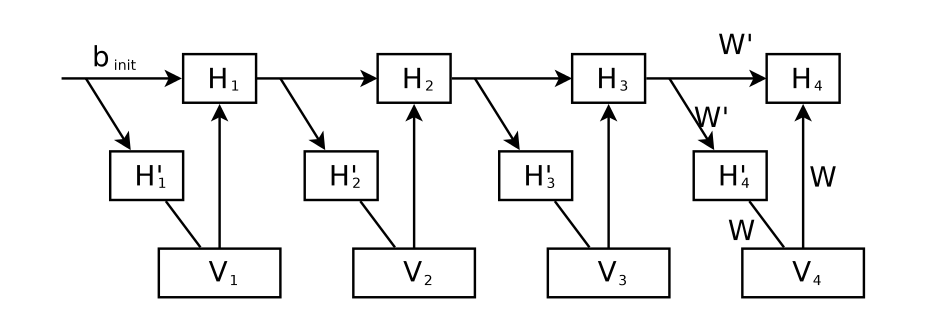
\includegraphics[scale=0.4]{Figures/RTRBM.png}
    \rule{35em}{0.5pt}
    \caption[RTRBM Graphical Model]{RTRBM Graphical Model}
    \label{fig:rtrbm}
\end{figure}

Boulanger-Lewandowski et al. change the RTRBM model to use a classical RNN to generate the biases for the RBM of the next time step (RNN-RBM \cite{boulanger2012modeling}): 
$$
\begin{array}{rcr}
    b_v^{(t)} & = & b_v + W_ {uv} u^{(t - 1)} \\
    b_h^{(t)} & = & b_h + W_{uh} u^{(t - 1)} \\
    u^{(t)} & = & tanh( b_u + W_{uu} u^{(t - 1)} + W_{vu}v^{(t)})
\end{array}
$$


\begin{figure}[htbp]
    \centering
    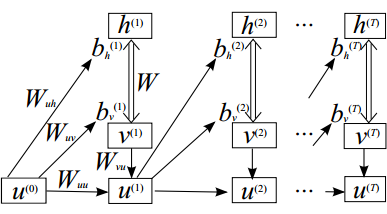
\includegraphics[scale=0.6]{Figures/RNNRBM.png}
    \rule{35em}{0.5pt}
    \caption[RNN-RBM Graphical Model]{RNN-RBM Graphical Model}
    \label{fig:rtrbm}
\end{figure}

This model was applied to the music score datasets and achieved the best results. However the model were not used for music generation specifically and this will be the focus of this project.

% Chapter Template

\chapter{ Study of the internal structure of a previously trained Recurrent Neural Network} % Main chapter title

\label{Chapter 3} % Change X to a consecutive number; for referencing this chapter elsewhere, use \ref{ChapterX}

\lhead{Chapter 3. \emph{Study of the internal structure of a previously trained Recurrent Neural Network}} % Change X to a consecutive number; this is for the header on each page - perhaps a shortened title

%----------------------------------------------------------------------------------------
%	SECTION 1
%----------------------------------------------------------------------------------------

%\section{State of the Art}

\section{Motivation}

In this chapter we study the internal structure of examples of previously trained recurrent neural networks in order to propose a practical improvement of the architecture for a given problem. The lack of understanding of the dynamics within a neural network and the progress of computation performance and implementation of Neural Netowrks led to accepting that the larger the network is, the better it is suited to obtain a better solution. Many techniques have been implemented in order to reduce the overfitting of these models that contains a large number of parameters such as Georges Hinton's dropouts for training Deep Feed-Forward Neural Networks. However, it seems rather unnatural to ommit the study of the internal structure of a network in the field of Deep Learning and especially for Recurrent Neural Network, where complex dynamics of the states can be observered. For example, in the classical model of a Recurrent Neural Network, the weight matrix is dense but if we observe the human brain, it is estimated that the number of neurons is approximatively $10^{11}$ and the number of synapses between $10^{14}$ and $10^{15}$, which means that the mean number of connections from a neuron to another is between $10^3$ and $10^4$ and therefore that the weight matrix is extreamly sparse. In this chapter we use graph theory techniques to perform an empirical study of different neural networks that have been previously trained on different problems. 

\section{Experiments}

\subsection{Problem}

The neural network is trained on a 100 timestep sequence of random binary number, where the goal is to memorize the first input given to the network. It contains 100 neurons and is trained using the Hessian Free Optimization method (HFO). This example use the Theano implementation of the HFO of Boulanger-Lewandowski \cite{boulanger2012modeling}. The network was trained for approximatly 8 hours on a 4 cores computer which gave a 0 error on the validation set as described on the Github repository of Boulanger-Lewandowski. In the end of the training we obtain the (100, 100) hidden-to-hidden weight matrix and perform the graph analyse on this matrix. This kind of memorization problem is typically hard for a recurrent neural network to learn, when its trained using stochastic gradient descent because it emphasizes the vanishing gradient problem. The relevant input is 100-timestep old, and therefore the weight matrix is multiplied a 100 times, before reading the output which will be small as a composant of the gradient, this problem demonstrates the importance of a 2-order optimization method for RNNs. 

\subsection{Plot of the RNN}

In order to display the RNN, we use two differents layouts, the nodes are represented with red dots, the connection are in blue when $w_{ij}  > t $ where t is a threshold ($ t=0.15$ for the following figures) and in black when $w_{ij} < - t$  :

\begin{itemize}
    \item The spring layout, where the positions of the nodes is calculated as if each connection was a spring which rigidity constrain is the weight of the connection ( or 2 particles with opposite charge for a negative weight. ) (ie minimizing the energy $$ E(x, y) = \sum_{i,j} w_{ij}(\sqrt{(x_i - x_j)^2 + (y_i - y_j)^2} - l)^2 $$ where $l$ is the default length of a connection. 
    \item The spectral layout \cite{koren2003spectral} that performs eigenanalyses of the Laplacian Matrix ($L$) of the Graph and uses the eigenvectors of L to display the nodes on the 2D plane. L is defined as $$ L = D - A $$ where A is the symmetrical Matrix $$ A = 0.5(W + W^\top) $$ (because the RNN is a directed Graph.) and D is the diagonal matrix such that :  $$ D_{ii} = \sum_j A_{ij} $$ 
        $L$ is a semi-definite symmetrical Matrix with zero row sums. Therefore there is a spectral decomposition of this Matrix with positive eigenvalues and its eigenvectors are orthogonal. The two (or more for a n-dim layout) eigenvectors corresponding to the smallest non-zero eigenvalues are kept and use as the x and y coordinates.  

        The Laplacian matrix has the following property : $$x^\top  L x = \sum_{i < j} A_{ij}(x_i - x_j)^2 $$
        Displaying the graph as follow is the solution of a minimization problem ie : For a 1-D layout minimizing the energy $E$ defined as follow : 
        $$ E(x) = \sum_{i,j} A_{ij} (x_i - x_j)^2 $$ where $x \in \mathbb{R} $ with a constrain on the variance of $x$ : $Var(x) = 1 $. 
        Minimizing this energy with a fixed variance will tend to make the edges as small as possible (with respect of the weights) and prevent all nodes to be on the same position. 
    This problem is equivalent to the following (when placing the mean of x to be null) : 
    $$ min_x x^\top L x $$
    given $ x^\top x = 1 $
    on the hyperplane $x^\top \dot 1_n = 0 $

    which corresponds to setting x to be the smallest normalized eigenvectors ($v_1$) (ie corresponding to the smallest non-zero eigenvalue) of L.
    The same reasonning can be applied to obtaining a k-dim layout, as the eigenvectors are orthogonals, we can resolve the same minimisation problem on the the subspace orthogonal to $v1$ for the second dimension ( which will be taking $y = v_2$) and so on. 
\end{itemize}


\begin{figure}[htbp]
    \centering
    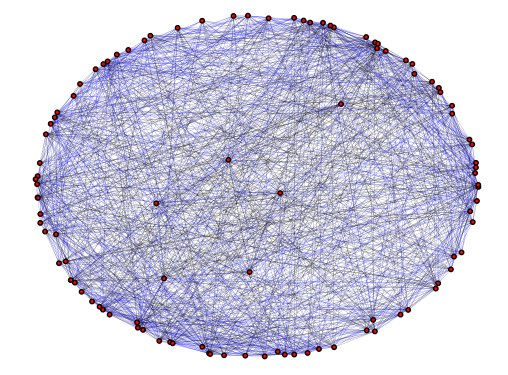
\includegraphics[scale=0.8]{Figures/weighted_graph_spring.png}
    \rule{35em}{0.5pt}
    \caption[Plot of the RNN using weights as springs]{Plot of the RNN using weights as spring}
    \label{fig:ring_lattice}
\end{figure}


\begin{figure}[htbp]
    \centering
    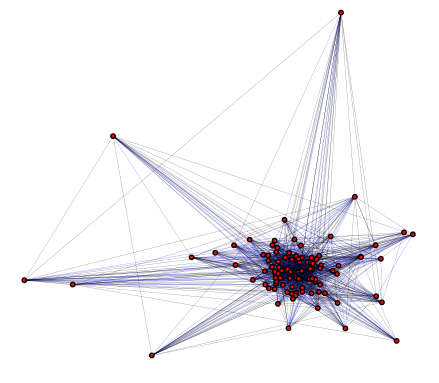
\includegraphics[scale=0.8]{Figures/weighted_graph_spectral.png}
    \rule{35em}{0.5pt}
    \caption[Plot of the RNN with spectral analyses of the Laplacian Matrix ]{Plot of the RNN with spectral analyses of the Laplacian Matrix}
    \label{fig:ring_lattice}
\end{figure}

We can observe that 5 nodes are on the periphery of the spectral graph, which means that they have small connection to the rest of the nodes (ie no strong connection to a cluster), whereas the other nodes have neighbors "strongly" attached to them. 

\subsection{Weight distribution}
It is also interesting to display the weight distribution : 

\begin{figure}[htbp]
    \centering
    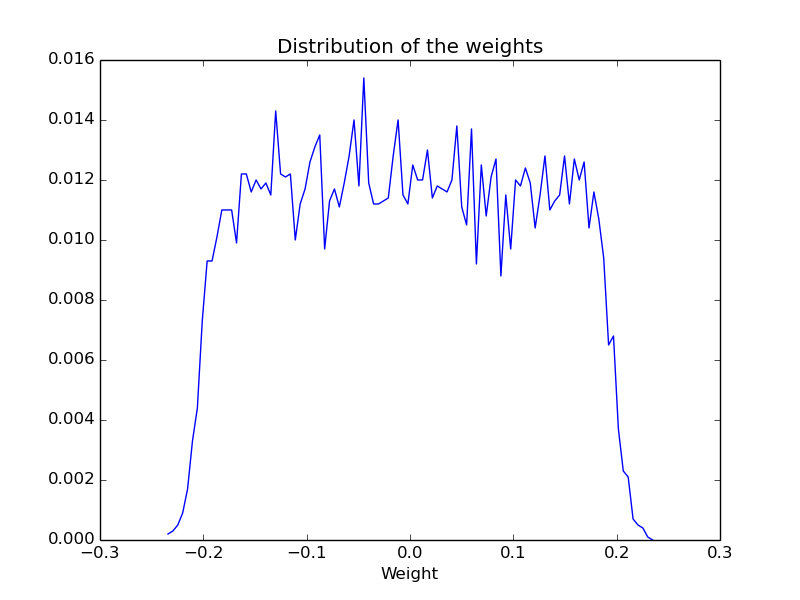
\includegraphics[scale=0.4]{Figures/weight_distribution.png}
    \rule{35em}{0.5pt}
    \caption[Weight distribution ]{Weight distribution}
    \label{fig:weight_dist}
\end{figure}

\begin{figure}[htbp]
    \centering
    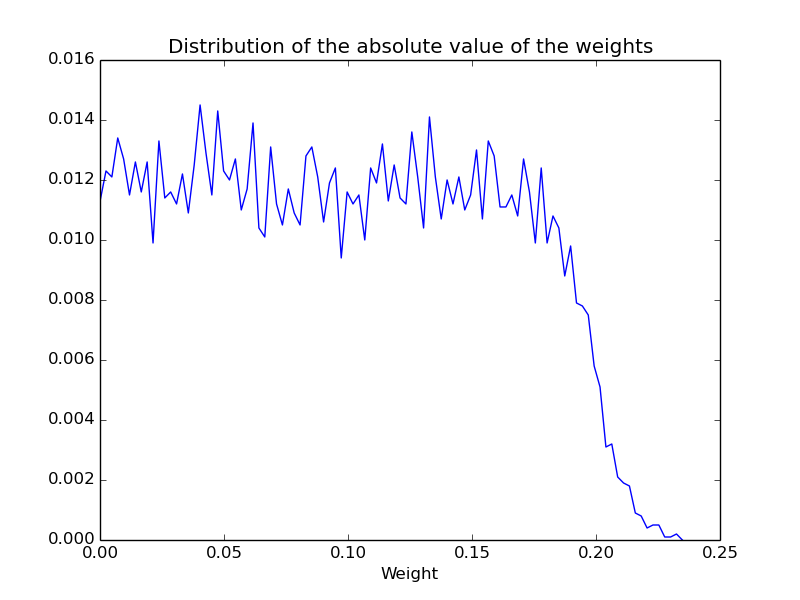
\includegraphics[scale=0.4]{Figures/abs_weight_distribution.png}
    \rule{35em}{0.5pt}
    \caption[Distribution of the absolute value of the weights]{Distribution of the absolute value of the weights}
    \label{fig:abs_weight_dist}
\end{figure}

We can observe a that the distribution is relativly symmetric and that most weights are within the interval $[-0.2;02] $

\subsection{Sums of weights}

It is also interesting to compute the sum of the absolute value of the weights of the input connections in the hidden matrix ( ie : the rows of $W_{hh}$) ($\sum_{in,}(Whh)$) and also the output connection ($\sum_{out,}(Whh)$) (ie the columns of t $W_{hh} $). A neuron without any influence on the network have ($\sum_{out,}(Whh) = 0$) and a neuron which state is constant has the $\sum_{in,}(Whh) = 0$. Therefore by studying this 2 sums, we can hope to determine if some neurons are useless, or in the opposite if one neuron should be cloned.
The following figures are the plot of these sums on the network. 

\begin{figure}[htbp]
    \centering
    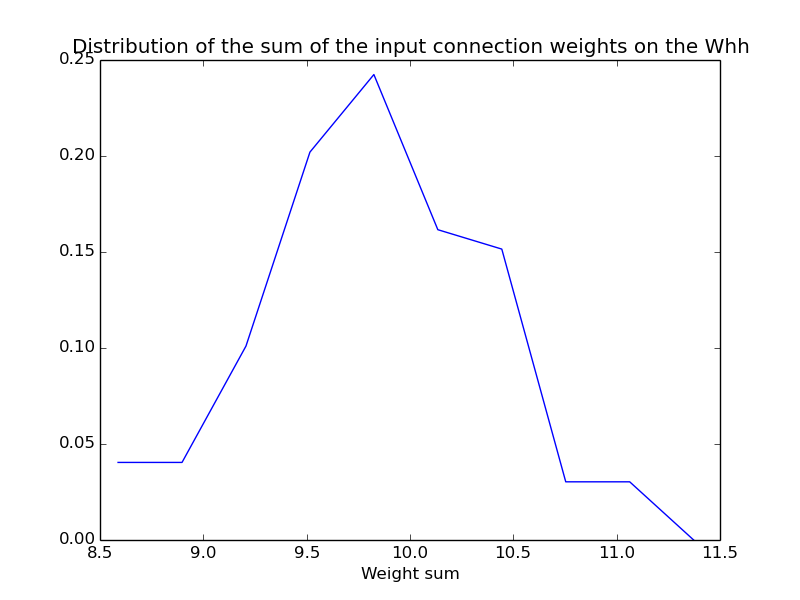
\includegraphics[scale=0.4]{Figures/input_sum_weight_distribution.png}
    \rule{35em}{0.5pt}
    \caption[Distribution of the sum of the input connection weights on Whh]{Distribution of the sum of the input connection weights on Whh}
    \label{fig:input_sum}
\end{figure}


\begin{figure}[htbp]
    \centering
    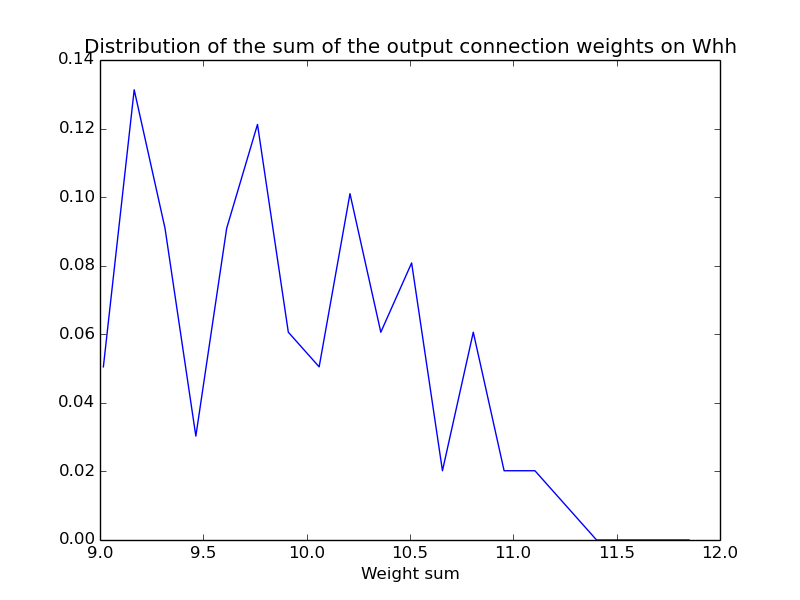
\includegraphics[scale=0.4]{Figures/output_sum_weight_distribution.png}
    \rule{35em}{0.5pt}
    \caption[Distribution of the sum of the output connection weights on Whh]{Distribution of the sum of the output connection weights on Whh}
    \label{fig:output_sum}
\end{figure}

A surprising result is that these two sums do not change as much as expected over the set of neurons : for all the neurons these two sums are within $[8.0; 12.0]$, it is therefore difficult two establish which neuron to remove based on this measure.

\subsection{Compairing neurons of the network.}

We can also directly measure the impact of a neuron on the network. By replacing all the inputs and output weights of the neuron with zeros, we destroy its impact on the RNN. It is then possible to test the network on a test set of sequence. We then display the results, that represent the percentage of errors on the test set. 

\begin{figure}[htbp]
    \centering
    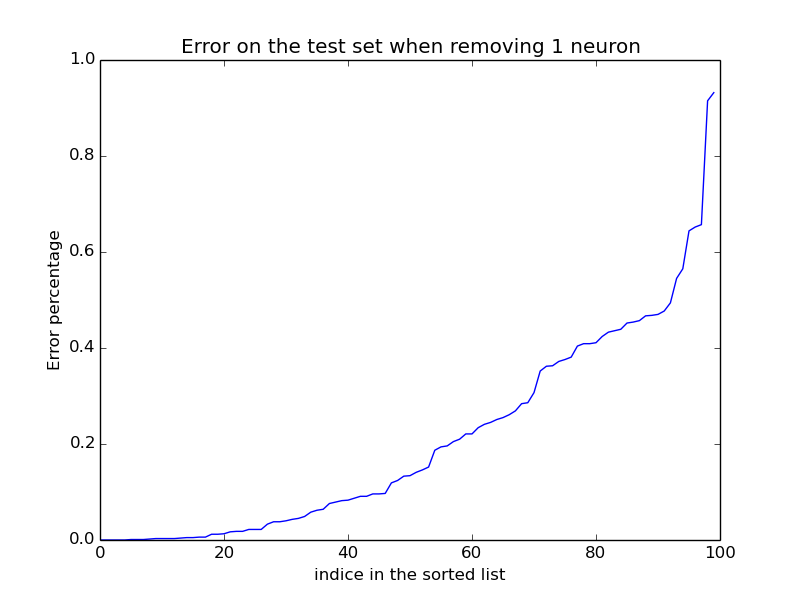
\includegraphics[scale=0.8]{Figures/error_test_set_remove_neuron.png}
    \rule{35em}{0.5pt}
    \caption[Error on the test set when removing 1 neuron]{Error on the test set when removing 1 neuron}
    \label{fig:error_one_neuron}
\end{figure}

In the figure \ref{fig:error_one_neuron} we display the sorted list of percentage error on the test set when removing 1 different neurons at each time. This figure demonstrate that the importance of the neurons in the network is very unequal. For $20$ neurons out of $100$, the network without this neuron the error rate will not exceed $3\%$ whereas if we remove only $1$ "important" neuron in the top $20$ , the network will have lesser performance than random guess ! This shows that the dynamics within a network can be perturbed easily only with a small modification of the architecture if this modification affects the wrong neurons. Another really interesting results that this graph shows is that the sum of the weights does not give a good approximation of the importance of a neuron's worth.

Using this measure, we can introduce an order relation $O$in the set of neuron : 

$$ N_i <= N_k \Leftrightarrow m(N_i) <= m(N_j) $$ where $m$ is a function that return the error percentage on the test set when removing a the neuron of the network.

In the following we compare this order relation with the ones obtained using other intrinsic metrics of the network. The goal is to find a way of knowing which neurons to remove in the network without "breaking" the dynamics involved so that the network is more efficient. In order to compare a metric with the $m$ we sort the set of neurons and compare the list of indices. 

$$ d(s , s') =  \sum_{i \in \mathbb{N}} {| s_i - s'_i|} $$

A low value of $d$ means that 2 metrics order the neurons similarly. Using $d$ with the previously defined order relation provides a benchmark for finding an approximation of the worth of a neuron in the network. In the following we present the results of different metrics on this benchmark.

The metrics that were tested on the network are : 
\begin{itemize}
    \item M1 : The sum of the absolute value of the in an out weights on the hidden-to-hidden connection
    \item M2 : The sum of the in an out weights on the hidden-to-hidden connection
    \item M3 : The absolute value of the sum of the in an out weights on the hidden-to-hidden connection
    \item M4 : The clustering index
    \item M5 : The absolute value of the ouput weight ( of the hidden to output matrix) 
    \item M6 : The absolute value of the input weight ( of the hidden to output matrix) 
    \item M7 : The sum of the two previous metrics.
\end{itemize}

All the metrics were normalized to be able to plot them with $m$
In the following graphs we ploted the metrics for the sorted list of neurons with $O$, as well as the value of $m$. 


\begin{figure}[htbp]
    \centering
    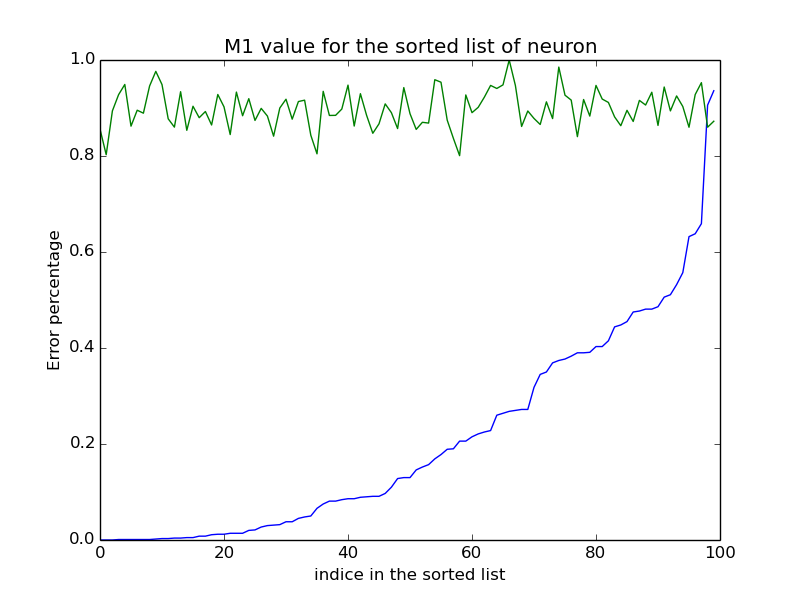
\includegraphics[scale=0.5]{Figures/m1.png}
    \rule{35em}{0.5pt}
    \caption[M1]{M1}
    \label{fig:m1}
\end{figure}


\begin{figure}[htbp]
    \centering
    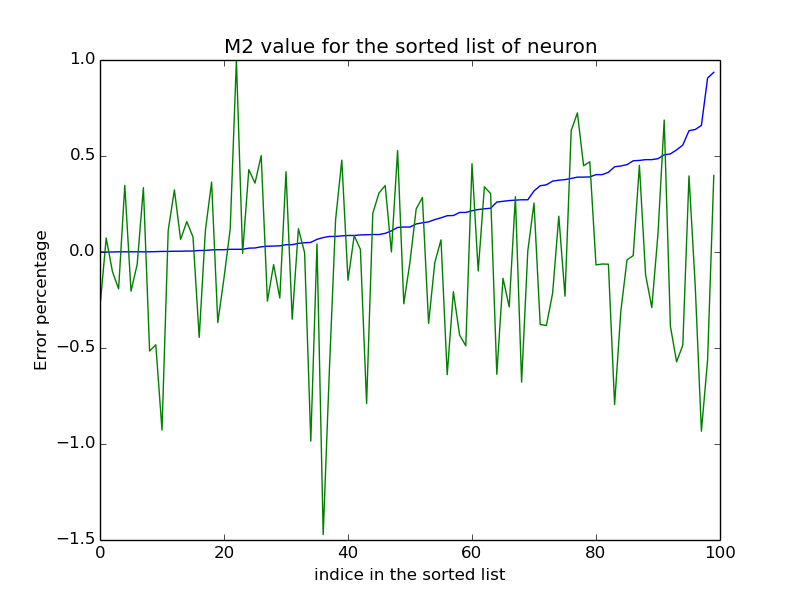
\includegraphics[scale=0.5]{Figures/m2.png}
    \rule{35em}{0.5pt}
    \caption[M2]{M2}
\label{fig:m2}
\end{figure}


\begin{figure}[htbp]
    \centering
    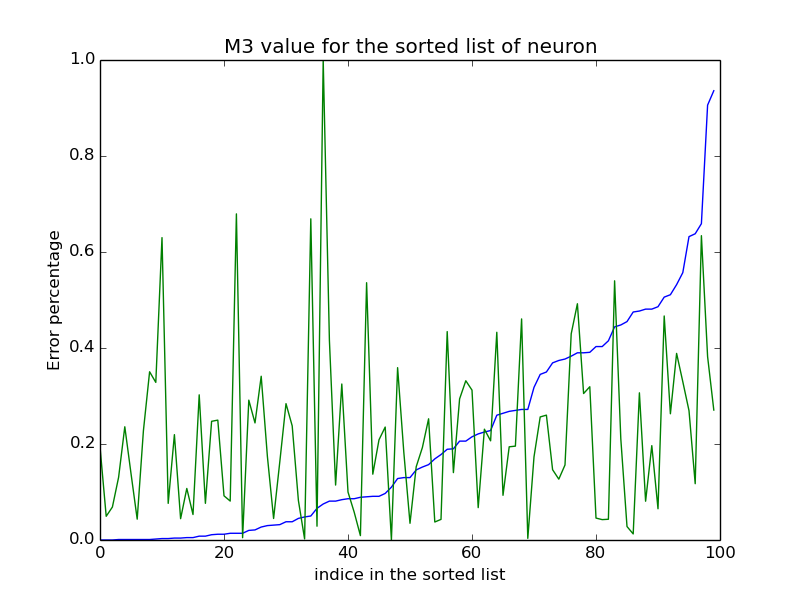
\includegraphics[scale=0.5]{Figures/m3.png}
    \rule{35em}{0.5pt}
    \caption[M3]{M3}
    \label{fig:m3}
\end{figure}


\begin{figure}[htbp]
    \centering
    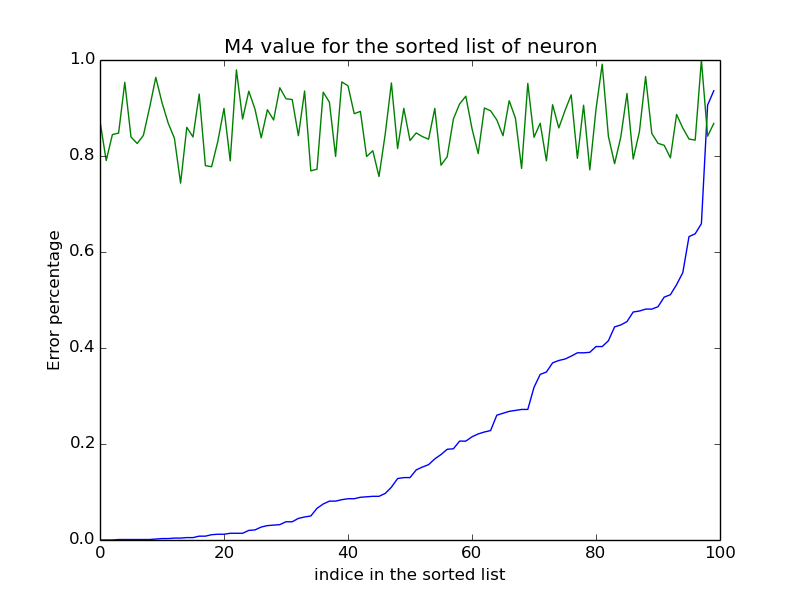
\includegraphics[scale=0.5]{Figures/m4.png}
    \rule{35em}{0.5pt}
    \caption[M4]{M4}
    \label{fig:m4}
\end{figure}


\begin{figure}[htbp]
    \centering
    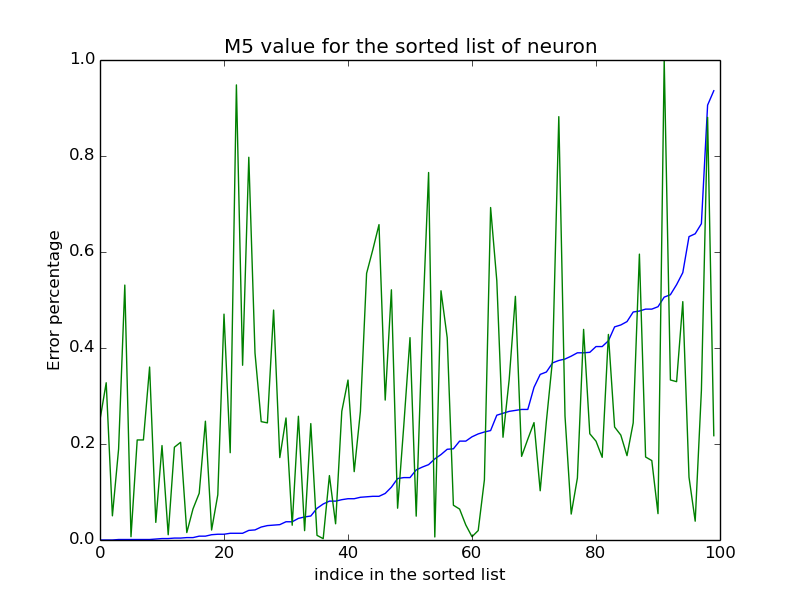
\includegraphics[scale=0.5]{Figures/m5.png}
    \rule{35em}{0.5pt}
    \caption[M5]{M5}
    \label{fig:m5}
\end{figure}


\begin{figure}[htbp]
    \centering
    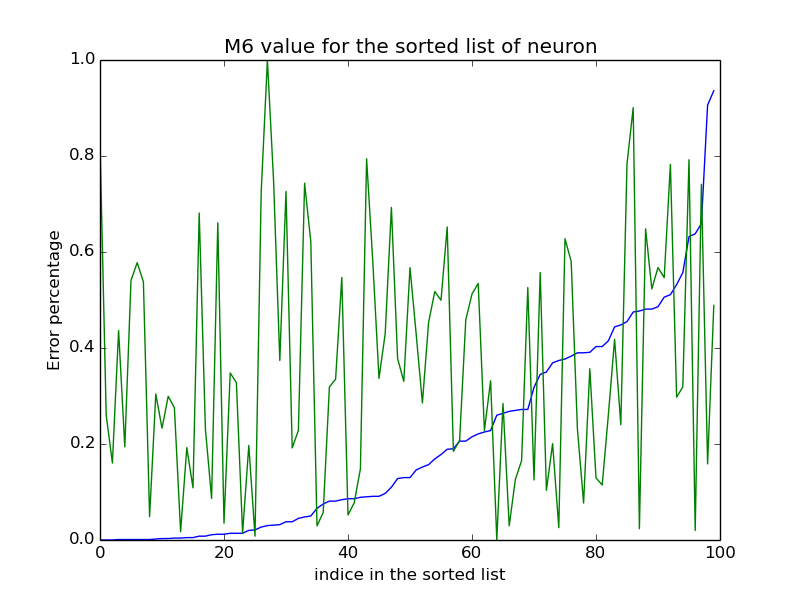
\includegraphics[scale=0.5]{Figures/m6.png}
    \rule{35em}{0.5pt}
    \caption[M6]{M6}
    \label{fig:m6}
\end{figure}


\begin{figure}[htbp]
    \centering
    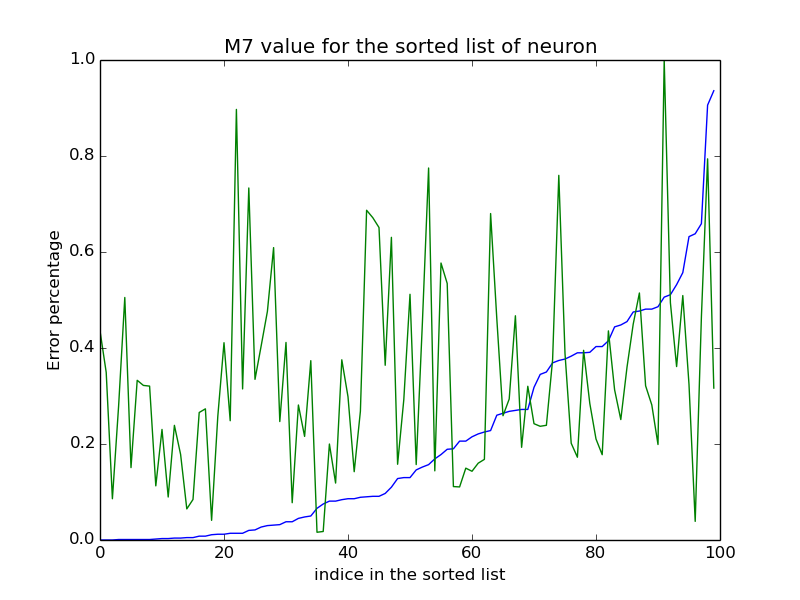
\includegraphics[scale=0.5]{Figures/m7.png}
    \rule{35em}{0.5pt}
    \caption[M7]{M7}
    \label{fig:m7}
\end{figure}


In order to make the figure \ref{fig:m4} we use the clustering index  : TODO ADD DESCRIPTION HERE


\begin{figure}[htbp]
    \centering
    \begin{tabular}{|l|l|}
        \hline
        M1 & 3118 \\ \hline
        M2 & 3294 \\ \hline
        M3 & 3512 \\ \hline
        M4 & 3388 \\ \hline
        M5 & 3244 \\ \hline
        M6 & \textbf{2944} \\ \hline
        M7 & 3402 \\
        \hline
    \end{tabular}
    \label{fig:metrics}
    \rule{35em}{0.5pt}
    \caption[Table presenting the value of d for the different metrics ]{Table presenting the value of d for the different metrics}
\end{figure}



\subsection{Compairing connections in the network.}

% Chapter Template

\chapter{ Self-Growing Recurrent Neural Network} % Main chapter title

\label{Chapter 2} % Change X to a consecutive number; for referencing this chapter elsewhere, use \ref{ChapterX}

\lhead{Chapter 2. \emph{Self-Growing Recurrent Neural Network}} % Change X to a consecutive number; this is for the header on each page - perhaps a shortened title

%----------------------------------------------------------------------------------------
%	SECTION 1
%----------------------------------------------------------------------------------------

%\section{State of the Art}

\section{Introduction}

In this Chapter, we introduce Self-Growing Recurrent Neural Network (SGRNN), which is a Recurrent Neural Network that change its architecture as well as its weights during learning. In the standard Recurrent Neural Network, the hidden-to-hidden weight Matrix ($W_{hh}$) is considered as a dense Matrix in the calculation. This means that each neuron is connected to all the other neurons and that each weight takes the same ammount of computation time to update. Therefore, the learning step in the hessian free optimization (HFO) or stochastic gradient descent compute an update for each elements of this weight matrix. However, from a biological perspective, it makes sense to restrict the connections of a neuron to neuron that are near it. Performing such a change in the architecture of a RNN, reduce the number of connections complexity from $n^2$ to $n$. The same observation can be made for inputs and outputs weights : All neuron connections to the inputs and the the outputs are not necessary. Such an architecture change can reduce the computation time for the same number of neurons. It can also provide a structure in the weights matrices to simplify the scalability and the implementation of this model on distributed systems, by performing a cluster analyses of the weight matrix.

\section{SGRNN}

The SGRNN structure is the same as the standard RNN. The difference come from the learning algorithm.

$$
\begin{array}{rcr} 
    h_0 & = & a(W_{hx}  * x_0 + b_{init} + b_h)  \\ 
    h_i & = & a(W_{hx}  * x_i + W _{hh} * h_{i-1} + b_h)  \\ 
    \hat{y}_i & = & a'(W_{yh} + b_y)

\end{array}
$$


\begin{algorithm}
    \caption{Learning algorithm}
    \begin{algorithmic}
    \STATE $ weightsInit() $
    \WHILE{$continueTraining$}
        \FOR{$i \in [1: nSteps]$}
            \STATE $HFOStep()$
        \ENDFOR
        \STATE $evolutionStep()$
        \STATE $reorderingStep()$
    \ENDWHILE
    
    \end{algorithmic}
\end{algorithm}

\subsection{Implementation of the Hessian Free Optimization step}
The Hessian Free Optimization \cite{martens2011learning} is implemented using the Theano library, that handle efficient symbolic differentiation (on GPU), especially for multi-dimensional arays, which makes it the perfect candidate to test and implement new models of Recurrent Neural Networks. Boulanger \cite{boulanger2012modeling} implemented the Hessian-Free optimization method with Martens \& Sutskever \cite{martens2011learning} improvements. 

Theano handles the differenciation automaticly once provided an expression such as the one defining RNNs. It is then possible to use the gradient function to obtain the gradient of this expression with respect to a list of parameters.

However the SGRNN step requires only to compute the gradient over the non-zero values in the sparse matrix representation of the hidden-to-hidden weight matrix. Therefore, we provide a mask to the RNN implementation, and we replace $W_{hh}$ with the hadamard product $M \circle W_{hh}$ , where $M$ is the mask, ie a binarry matrix that contains $1$ where there is a connection between neurons and $0$ elsewhere. Using this trick it is possible to use the classical Hessian free optimization (or a stochastic gradient descent) as the gradient of the network in respect to $Whh_{ij}$ is guaranted to be null if there is no connection between neuron $i$ and $j$. 


\subsection{Weights Initialization}

    In a standard RNN, the weight matrices are randomly initialized, in order to prevent symmetry that could not be broken during the learning phase within the model. For SGRNN we initialize the RNN with a small number of neurons using a K-band matrix with the top right and bottom left corner also filled, ie a sparse matrix, with non-zero weights on the diagonal and on the K diagonals on either side of the matrix as well as on the K diagonals in both top-left and bottom-right corner.

$$Whh_{ij} = 0 if \exists t \in \mathbf{N}, abs(i - j - t * n) < k $$ where $n$ is the number of neurons.

This weight matrix initialize the Neural Network as a ring lattice with self connections. 

TODO CHANGE PICTURE WITH SELF CONNECTIONS.

\begin{figure}[htbp]
    \centering
    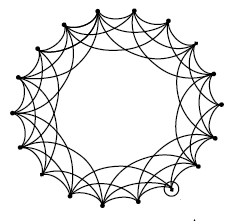
\includegraphics[scale=0.7]{Figures/ring_lattice.png}
    \rule{35em}{0.5pt}
    \caption[A ring lattice]{A ring lattice}
    \label{fig:ring_lattice}
\end{figure}

We initialize the input and output weight matrices as well as the biases using the same process as in the RNN model. 
The parameters of the model for the hessian free optimization step are only the non-zero weights. 

\subsection{Evolution Step}

The evolution step consist of three different steps:
\begin{itemize}
    \item Adding weights: if two consecutive weights ($ab$, $bc$) are above a weight treshold, we diminush them by half and create a new connection ($ac$)
    \item deleting weights that are near zero
    \item Adding neurons: We duplicate with a small noise (on the connections to break the symmetry) the neuron with the highest clustering coefficient. 
\end{itemize}


\subsection{Reordering Step}
    The goal of the reordering step is to switch neurons position in $Whh$ so that the matrix keeps the same shape as in the initialization step. 










% Chapter Template

\chapter{Conclusion and Future Work} % Main chapter title

\label{Chapter 5} % Change X to a consecutive number; for referencing this chapter elsewhere, use \ref{ChapterX}

\lhead{Chapter 5. \emph{Conclusion and Future Work}} % Change X to a consecutive number; this is for the header on each page - perhaps a shortened title

%----------------------------------------------------------------------------------------
%	SECTION 1
%----------------------------------------------------------------------------------------

%\section{State of the Art}

\section{Conclusion} 
    In the first part of this project we conducted an empiracl study on a trained RNN. This study showed that the current indicators such as the sum of the weights connected to a neuron or the clustering coefficient used in graph theory do not provide meaningful information on the network. The dynamics involved within a RNN are complex to modelize. In particular tentatives to order the neurons based on their importance is hard when considering only the graph structure without a validation dataset. We also proved similar unnatural behavior concerning the connections weights: if a near-zero weight is less likely to be important for the network, a large weight in a connection does not necessary means that this connection is important. Finally we showed that using a dense weight matrix for a RNN was not necessary on the memorization problem.  
 

    The result obtained in the first chapter led to the design of Self Growing Recurrent Neural Network (SGRNN) a network that change its weights as well as its architecture during learning. By selecting neurons to be removed and performing a cloning of neurons, it is possible to dynamicly adjust the number of neurons for a given problem. This technique can also be used for pre-training a RNN. 


\section{Future Work}

The empirical work presented in Chapter 3, confirmed that the dynamics within RNN is complex and that works remains to grasp the interactions between neurons. In particular finding a way of knowing which neuron or cluster of neuron is important during computation for RNN might lead to significant progress in the training of such a network. It could potentially also have applications in neuroscience. As some of the indicators that seens "natural" failed to do this task, it would be interesting to apply a Machine Learning technique directly on the network to predict the score (or a metric with the same order relation) that the network obtains on a validation set, without this particular neuron or group of neurons. The same approach could also be applied directly on connections. 

Also, based on the results obtained in this project, using sparse matrix respresentation could lead to good performance. Implementing an efficient Hessian Free Optimization algorithm for sparse matrix RNN is still needed, as we used "mask" to simulate sparse weight matrix in this project.

Finally the flexibility of the technique used in SGRNNs to add and remove neurons could benefit from a better understanding of RNNs, especially in the choice of neurons to be cloned as we rely on the assumption that an important neuron should be cloned. This assumption would require to study the performance of the network to learn faster in the next learning steps, which requires a substantial ammount of computation. However, this is quite similar to the assumption used in genetic algorithms, where the cross-over is an operation between 2 "good" candidates.    

%\input{Chapters/Chapter4} 
%\input{Chapters/Chapter5} 
%\input{Chapters/Chapter6} 
%\input{Chapters/Chapter7} 

%----------------------------------------------------------------------------------------
%	THESIS CONTENT - APPENDICES
%----------------------------------------------------------------------------------------

\addtocontents{toc}{\vspace{2em}} % Add a gap in the Contents, for aesthetics

%\appendix % Cue to tell LaTeX that the following 'chapters' are Appendices

% Include the appendices of the thesis as separate files from the Appendices folder
% Uncomment the lines as you write the Appendices

%% Appendix A

\chapter{Appendix Title Here} % Main appendix title

\label{AppendixA} % For referencing this appendix elsewhere, use \ref{AppendixA}

\lhead{Appendix A. \emph{Appendix Title Here}} % This is for the header on each page - perhaps a shortened title

Write your Appendix content here.
%\input{Appendices/AppendixB}
%\input{Appendices/AppendixC}

\addtocontents{toc}{\vspace{2em}} % Add a gap in the Contents, for aesthetics

\backmatter

%----------------------------------------------------------------------------------------
%	BIBLIOGRAPHY
%----------------------------------------------------------------------------------------

\label{Bibliography}

\lhead{\emph{Bibliography}} % Change the page header to say "Bibliography"

\bibliographystyle{unsrtnat} % Use the "unsrtnat" BibTeX style for formatting the Bibliography

\bibliography{Bibliography} % The references (bibliography) information are stored in the file named "Bibliography.bib"

\end{document}
